\section{Introduction}
\label{sec:intro}

As the Internet continues to control and define more aspects of the physical world, the consequences of Internet attacks also continue to scale. Network attacks, once an annoyance or hassle, can now translate into a loss of money, a source of physical harm, or even widespread chaos. In the past few years alone, we have seen network attacks destroy nuclear reactor development \cite{stux}, hold hospitals ransom \cite{ransom}, and even control moving vehicles \cite{carhack}. 

An area increasingly targeted by attackers is the Internet of Things. It is hard to imagine the influence of computer networks and the prevalence of the Internet ever waning. Therefore, creating permanently secure and stable networks is a major technical problem that must be solved before the Internet of Things firmly takes hold. A significant challenge is that a significant segment of the IoT deployments target home deployments.  Whereas enterprises have the resources and IT staff to manage security (and still get attacked), home users do not have such resources.  We propose that users in the cyber world need the digital equivalent of a physical Home Security System -- such as provided by ADT \cite{adt}, which monitors physical aspects (\eg door open) of the home and automatically defends against intrusions. 

%Perhaps a good source of inspiration for the problem of securing these innumerable, complex networks is the physical layer of the Internet itself. Despite the daunting physical, link, and protocol issues of running cables throughout the countries of the world, it is amazing that modern users do not even need to know how the Internet works to benefit from its many services.  Network security should similarly be invisible to the average user.  


\begin{figure}
    \centering
    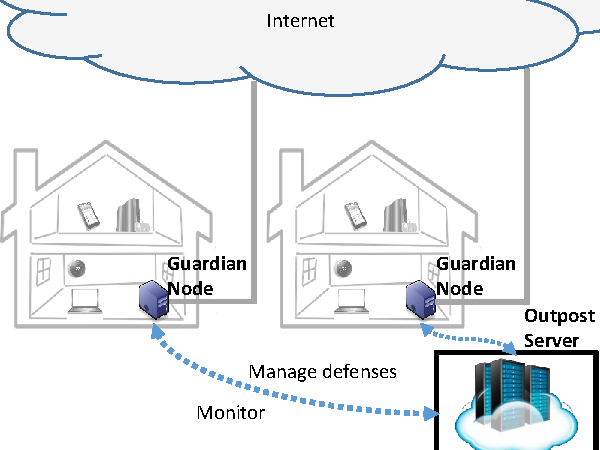
\includegraphics[width=0.87\columnwidth]{figs/highlevel.pdf}
    \caption{CommunityGuard architecture.}
    \label{fig:arch}
\end{figure}



In this paper we present CommunityGuard (illustrated in Figure~\ref{fig:arch}), a system which automatically protects home users from external attacks (much like a home security system), helps prevent home users from unwittingly being used to launch attacks on others, and provides a means for home users to look out for each other (similar to neighborhood watches where people can report suspicious activity to help their neighbors).  This is all possible with the combination of network functions virtualization to launch monitoring and defenses where needed, and software defined networking to remotely manage the configuration.  In essence, CommunityGuard is (in one deployment model) simply a device that resides between a home router and the cable modem, which connects to a cloud system that automatically monitors for suspicious activity and deploys the appropriate response.  Through relying on the collaborative aspects of this network of devices, CommunityGuard has wide visibility that enables it to catch ever-more complicated malware and threats, and ultimately block malicious traffic from ever reaching its intended destinations. 

As a demonstration of the power of CommunityGuard, we focus on Distributed Denial of Service (DDoS) attacks, which are poised to grow dramatically in damage and scale.  DDoS is a common network attack in which a user attempts to make an extremely high number of resource requests in a short time in order to prevent others from accessing the resource. The strength of a DDoS attack is proportional to the number of resources an attack can leverage against its opponent and the time for which they can sustain their requests. For this reason, the Internet of Things looming on the horizon (which promises as much as 400 zettabytes of data by 2018 \cite{zetta}) has already given attackers a huge advantage in sustaining record-breaking DNS attacks against increasingly worrying targets. In events such as the attack on Dyn \cite{dyn}, a moderate amount of traffic passed from an unprecedented number of unique devices (mainly IoT cameras) to create an overwhelming force.  In this paper, we demonstrate the use of CommunityGuard for defeating these potentially-enormous DDoS attacks by stopping the traffic at the weaker end of its path -- the source subnet (home networks). 




